\chapter{Teori}
\label{cha:theory}


%% Vad behöver läsaren veta för att förstå resten av rapporten? %%

The main purpose of this chapter is to make it obvious for
the reader that the report authors have made an effort to read
up on related research and other information of relevance for
the research questions. It is a question of trust. Can I as a
reader rely on what the authors are saying? If it is obvious
that the authors know the topic area well and clearly present
their lessons learned, it raises the perceived quality of the
entire report.

After having read the theory chapter it shall be obvious for
the reader that the research questions are both well
formulated and relevant.

The chapter must contain theory of use for the intended
study, both in terms of technique and method. If a final thesis
project is about the development of a new search engine for
a certain application domain, the theory must bring up related
work on search algorithms and related techniques, but also
methods for evaluating search engines, including
performance measures such as precision, accuracy and
recall.

The chapter shall be structured thematically, not per author.
A good approach to making a review of scientific literature
is to use \emph{Google Scholar} (which also has the useful function
\emph{Cite}). By iterating between searching for articles and reading
abstracts to find new terms to guide further searches, it is
fairly straight forward to locate good and relevant
information, such as \cite{test}.

Having found a relevant article one can use the function for
viewing other articles that have cited this particular article,
and also go through the article’s own reference list. Among
these articles on can often find other interesting articles and
thus proceed further.

It can also be a good idea to consider which sources seem
most relevant for the problem area at hand. Are there any
special conference or journal that often occurs one can search
in more detail in lists of published articles from these venues
in particular. One can also search for the web sites of
important authors and investigate what they have published
in general. 

This chapter is called either \emph{Theory, Related Work}, 
\emph{Related Research}. Check with your supervisor.
\newpage










\section{Punktmoln}
På senare år har det blivit möjligt att representera objekt i form av ett 3D-representerat punktmoln. Detta har blivit möjligt på grund av utvecklandet av kameror samt laserskannrar. Ett punktmoln är alltså en mängd av punkter i ett tredimensionellt koordinatsystem som representerar ett objekt, se figur \ref{fig:point_cloud_torus}. Punkterna i punktmolnet representerar ofta de yttre kanterna av objektet.

\begin{figure}[H]
	\centering
	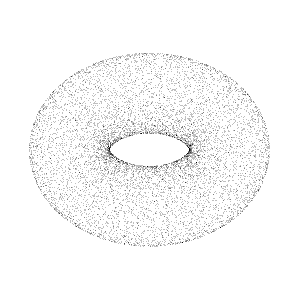
\includegraphics[width=50mm]{figures/Point_cloud_torus.png}
	\caption{Ett punktmoln som representerar ett torus objekt.}
	\label{fig:point_cloud_torus}
\end{figure}


\section{Point Cloud Library}
Point Cloud Library (PCL) är ett bibliotek till C++. PCL presenterar ett avancerat tillvägagångssätt angående ämnet 3D-uppfattning och är tänkt att ge stöd för vanliga 3D-byggstenar som olika applikationer behöver. Biblioteket innehåller algoritmer för att lösa problem med:

\begin{itemize}
	\item Filtrering
	\item Registrering
	\item Segmentering
	\item Modell anpassning
	\item ytrekonstruering
	\item funktionskalkylering
\end{itemize}

PCL är alltså ett bibliotek avsett att ge stöd till att behandla punktmolnsdata, iform av olika bearbetningsalgoritmer.
\section{Registrering}
\section{Meshning}
Att 



\section{Hållbar utveckling}
Hållbar utveckling är en relevant aspekt i dagens utveckling av programvaror eftersom de används kontinuerligt av samhället. Effekterna som en programvara bidrar med i samhället beror på hur den har producerats och hur den används av konsumenterna. Detta gör att effekterna av som en programvara bidrar med i samhället kan vara både positiva men också djupt negativa \cite{raturi2014developing}. Hållbarhet definieras som \textit{förmåga att uthärda} och \textit{bevara funktionen hos ett system under en utsträckt tidsperiod}. Att analysera hållbarhet hos ett mjukvarusystem innebär för de som utvecklar systemet att väga in dessa fyra områden i åtanke \cite{lago2015framing}:

\begin{itemize}
	\item Ekonomiskt -  Systemet ska bevara kapital och värde.
	\item Socialt - Systemet ska underhålla samhället.
	\item Miljö - Systemet ska skydda mänskliga välfärden genom att skydda naturens tillgångar.
	\item Tekniskt - Systemet ska utvecklas för att stödja långtidsanvändning.
\end{itemize}

Ett system för 3D-kopiering har många positiva effekter på samhället. Systemet gynnar framförallt miljön eftersom att tillverka en önskad produkt istället för att köpa en fabrikstillverkad sparar avsevärt på naturens tillgångar. Dels kommer 3D-kopieringssystemet att att använda mindre energi och dessutom kommer transporterna till och från affären att minska, vilket leder till mindre koldioxidutsläpp. Kreiger \cite{kreiger2013environmental} har gjort en studie där han skriver ut 3D-produkter i plast och jämför kostnaden för att tillverka produkter av plast i en fabrik. Med kostnaden menas den energi som går åt från råmaterial till färdig produkt samt kostnaden som går åt för transport. Det visar sig att tillverka en produkt i en 3D-skrivare kräver mellan 41 till 64 procent mindre energi än att fabrikstillverka produkten. Förklaringen till detta är att produkter som skrivs ut i en 3D-skrivare kan göras mer ihåliga och således kräver de också mindre material. 

Det finns dessutom relaterade studier som visar att det blir billigare att skriva ut en produkt i en 3D-skrivare istället för att köpa en fabrikstillverkad \cite{wittbrodt2013life}. Det här främjar samhället i positiv beaktning eftersom det helt enkelt blir billigare för konsumenter att införskaffa sig de produkter de önskar. 

\subsection{Förbättringspunkter till vårat system}
Vårat system för 3D-kopiering är som tidigare nämnts ett generellt bra system för att främja hållbar utveckling. Det finns däremot en del aspekter som skulle kunna gjorts annorlunda vid systemets uppbyggnad för att ytterligare främja hållbar utveckling. För att utveckla detta har vi valt att titta på hur våra krav framställdes, närmare bestämt besvara dessa frågor:

\begin{itemize}
	\item Hur skulle vi kunna göra annorlunda i kravprocessen?
	\item Vad har vi tagit hänsyn till i kravprocessen?
	\item Hur kan vi bedöma de krav vi satt på systemet med hållbar utveckling i åtanke?
\end{itemize}
Vid framställning av kraven till systemet fanns det inga tankar på att ta fram krav som främjar hållbar utveckling, det på grund av att ingen i projektgruppen hade erfarenheter från hållbar utveckling tidigare och således inte någon tanke på det. Vid framtagning av krav till systemet har alltså ingen hänsyn tagits till att främja hållbar utveckling. Det som har tagits hänsyn till i kravprocessen är endast funktionaliteten av systemet. Att utveckla icke funktionella krav för att främja denna aspekt är något som vi kunnat gjort annorlunda, det är också ett bra tillvägagångssätt enligt Raturi \cite{raturi2014developing}. 

En förbättring som vi kunde gjort är att systemet ska ha ett icke funktionellt krav att systemets beräkningar får ta en viss maximal tid. Detta är bra för energi- och miljösynpunkt eftersom hög processoranvändning under en lång tid leder till hög energiförbrukning för systemet. Det finns även en relation mellan hur systemet energianvändningen påverkas av hårdvaran i systemet. Den största energianvändande komponenten är processorn och därför skulle systemet även kunna ha ett icke funktionellt krav att optimera processoranvändningen, detta leder till energianvändningen för systemet minskar vilket är bra ur miljösynpunkt. Enligt Fan, Weber och Barroso \cite{fan2007power} ökar energiförbrukningen linjärt med processoranvändningen, detta är inte helt rättvisande och beror givetvis på vilken processor som används. 

För vårat system innebär det här att vi skulle vilja kombinera dessa två aspekter till ett gemensamt icke funktionellt krav. En kombination av dessa innebär att vi som grupp skulle behövt göra en studie över hur vi kan optimera processoranvändningen med avseende på energiförbrukning samtidigt som systemet inte får för lång körtid. Det optimala ur energispar synpunkt kanske skulle vara att låta systemet använda 70\% av processorn och istället få lite längre körtid. Detta är någonting som vi skulle kunna undersökt i förstudiefasen för senare användning till kravprocessen.

För att bedöma de krav som vi har med hållbar utveckling i åtanke kommer endast de krav som inte har med kärnfunktionaliteten att göra bedömas, eftersom de är nödvändiga för systemets funktionalitet. Andra krav bedöms ur energisynpunkt, om koden är tillräckligt optimerad för att uppfylla kravet eller om det blir för tungt beräkningsmässigt som gör att kravet inte uppfylls. Det skulle även vara möjligt att sätta upp icke funktionella krav med avseende på det sociala området som gör att användaren känner sig tillfredsställd med produkten och på så vis underhåller samhället. Detta bedöms genom att testa systemet med några användare och se huruvida det uppfyller användarens förväntningar eller inte. 


%%%%%%%%%%%%%%%%%%%%%%%%%%%%%%%%%%%%%%%%%%%%%%%%%%%%%%%%%%%%%%%%%%%%%%
%%% theory.tex ends here
